\chapter{T-dualité, D-branes et théorie de jauge}

\lectureoverview{La T-dualité établit d’abord une équivalence exacte entre les cordes fermées sur des cercles de rayons (R) et \(\alpha'/R\). La quantité de mouvement et l’enroulement échangent leurs rôles, de même que les dérivées de la feuille d’univers \(\partial_\tau Y\) et \(\partial_\sigma Y\), ainsi que les vecteurs d’espace-temps issus de \(G_{\mu 5}\) et \(B_{\mu 5}\). Lorsqu’on applique la même transformation à une corde ouverte, une condition aux limites de Neumann devient une condition de Dirichlet. L’extrémité doit alors se trouver sur une D-brane dynamique. Les cordes ouvertes confinées à une seule brane produisent une théorie de jauge abélienne à basse énergie ; celles qui relient un empilement de branes portent deux étiquettes d’extrémité et produisent une théorie de jauge non abélienne. Une D-string qui se termine sur une D3-brane fournit le monopôle magnétique correspondant.}

\section{Pourquoi revenir à la T-dualité ?}

Nous avons déjà rencontré la T-dualité, mais nous y revenons pour une raison précise. Elle fut l’un des indices montrant que la théorie des cordes contenait bien davantage que des cordes perturbatives. Une fois comprises ses conséquences pour les cordes ouvertes, elle a conduit aux D-branes ; celles-ci sont ensuite devenues un moyen de construire et d’étudier des théories quantiques des champs. Le but de ce cours n’est donc pas simplement de répéter le slogan selon lequel un petit cercle équivaut à un grand cercle. Nous allons reconstruire l’argument avec assez de soin pour voir comment ce slogan impose l’existence de nouveaux objets physiques dans la théorie.

Le cadre le plus simple est celui de la compactification toroïdale. Un tore de dimension un est un cercle. Un tore de dimension deux peut être représenté par un parallélogramme dont les côtés opposés sont identifiés, et un tore de dimension trois par un parallélépipède dont les faces opposées sont identifiées. La même construction se poursuit en dimensions supérieures. Nous ne garderons qu’une coordonnée spatiale compacte, notée \(Y\), et une coordonnée non compacte représentative, notée \(X\). Le temps est présent, mais n’apparaît pas dans les schémas au tableau.

Adoptons la convention usuelle
\begin{equation}
  Y\sim Y+2\pi R,
  \label{eq:l10-circle-identification}
\end{equation}
de sorte que \(R\) soit le rayon et \(2\pi R\) la circonférence. Dans ce cours, la taille de la direction compacte est souvent désignée simplement par \(r\), en omettant les facteurs de \(2\pi\) et \(\alpha'\). Nous conserverons les facteurs conventionnels dans les démonstrations et indiquerons les unités du cours lorsqu’elles seront utiles.

Dans la première moitié de la discussion, les cordes sont fermées et orientées. Une orientation est une flèche intrinsèque tracée le long de la corde. Inverser toutes les flèches partout ne changerait aucune expérience ; ce qui importe, c’est l’orientation relative de deux cordes. Lors d’une scission ou d’une fusion, les flèches doivent se raccorder de façon continue. C’est le premier indice de l’apparition d’une quantité signée et conservée.

\begin{figure}[H]
  \centering
  \includegraphics[width=0.72\textwidth]{lecture_10_figure_01.png}
  \caption{Deux cordes fermées dont les orientations relatives sont indiquées au tableau. L’orientation doit rester continue lors des scissions et des fusions.}
  \lectureframe{00:05:40}
  \label{fig:l10-oriented-closed-strings}
\end{figure}

\begin{classroomqa}
\audiencequestion{Si la coordonnée sur la feuille d’univers varie de
\(\sigma=0\) à \(2\pi\), la corde a-t-elle déjà fait un tour complet dans la direction compacte ? \lecturetimestamp{00:08:42}}
\lecturerresponse{Non. La coordonnée \(\sigma\) repère les points le long de la corde ; elle ne repère pas les positions dans l’espace compact. Toute corde fermée possède un paramètre périodique \(\sigma\), qu’elle soit enroulée ou non. L’analogie avec un élastique est utile : on peut numéroter les molécules le long d’un élastique même s’il n’est enroulé autour de rien. L’enroulement est une propriété de l’application \(Y(\tau,\sigma)\), et non du seul paramètre \(\sigma\).}
\end{classroomqa}

\begin{classroomqa}
\audiencequestion{La taille de la direction compacte doit-elle aussi être la même pour toute valeur de la grande coordonnée \(X\) ? \lecturetimestamp{00:10:00}}
\lecturerresponse{Pas dans une compactification dynamique générale. Nous commençons par un cercle de rayon fixe, car c’est le fond le plus simple. Plus tard, la composante \(G_{55}\) deviendra un champ scalaire dont la valeur mesure la taille locale de la cinquième direction ; cette taille pourra donc varier dans l’espace-temps ordinaire.}
\end{classroomqa}

\section{L’enroulement est conservé même lorsque les cordes se reconnectent}

Une corde non enroulée peut se déplacer dans la direction compacte sans s’y enrouler. Une corde enroulée est différente : lorsque \(\sigma\) parcourt une fois la corde fermée, l’application d’immersion \(Y(\tau,\sigma)\) progresse d’une ou plusieurs périodes du cercle compact. Comme la corde est orientée, cette progression est signée. Une corde peut s’enrouler dans le sens positif ou dans le sens négatif.

La loi de conservation apparaît le plus clairement dans les schémas de fusion. Prenons une corde d’enroulement \(+1\) et une autre d’enroulement \(-1\). Leurs segments compatibles peuvent se reconnecter. La configuration obtenue a un enroulement total nul et peut être déformée en une corde non enroulée. Le schéma au tableau représente précisément cette reconnexion d’orientations opposées.

\begin{figure}[H]
  \centering
  \includegraphics[width=0.72\textwidth]{lecture_10_figure_02.png}
  \medskip

  \begin{tikzpicture}[x=1cm,y=1cm,>=Latex]
    \draw[thick] (-4.0,0.3) circle (0.65);
    \draw[->,thick] (-4.55,0.58) arc (150:-145:0.65);
    \node at (-4.0,-0.65) {$w=+1$};
    \draw[thick] (-2.0,0.3) circle (0.65);
    \draw[<-,thick] (-2.55,0.58) arc (150:-145:0.65);
    \node at (-2.0,-0.65) {$w=-1$};
    \node at (-3.0,0.3) {$+$};
    \draw[->,thick] (-1.0,0.3) -- (0.3,0.3);
    \draw[thick] (1.4,0.3) ellipse (0.95 and 0.55);
    \node at (1.4,-0.65) {$w_{\rm total}=0$};
  \end{tikzpicture}
  \caption{Des enroulements opposés se reconnectent en une configuration d’enroulement total nul. Le schéma du bas est une reconstruction fidèle de la manipulation au tableau, et non un second processus dynamique.}
  \lectureframe{00:13:20}
  \label{fig:l10-opposite-winding}
\end{figure}

Reprenons maintenant l’expérience avec deux cordes de même orientation. Elles peuvent fusionner, mais elles ne peuvent pas se désenrouler. La corde obtenue porte un enroulement double de celui de chacune des cordes initiales. Le nombre de cordes connectées a changé ; l’enroulement total, lui, n’a pas changé.

\begin{figure}[H]
  \centering
  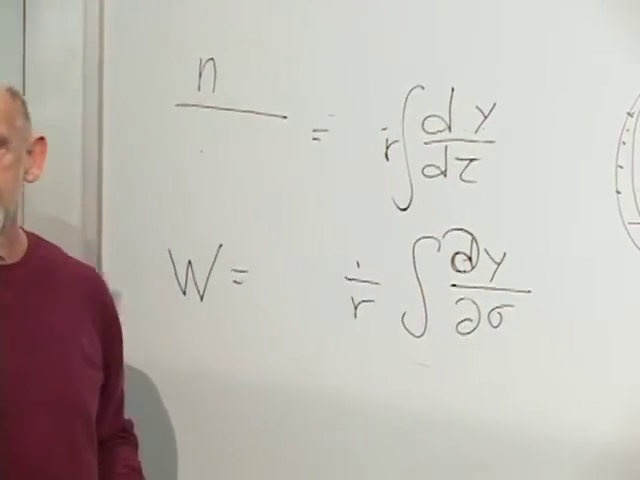
\includegraphics[width=0.72\textwidth]{lecture_10_figure_03.png}
  \medskip

  \begin{tikzpicture}[x=1cm,y=1cm,>=Latex]
    \draw[thick] (-4.0,0.3) circle (0.65);
    \draw[->,thick] (-4.55,0.58) arc (150:-145:0.65);
    \node at (-4.0,-0.65) {$w=+1$};
    \draw[thick] (-2.0,0.3) circle (0.65);
    \draw[->,thick] (-2.55,0.58) arc (150:-145:0.65);
    \node at (-2.0,-0.65) {$w=+1$};
    \node at (-3.0,0.3) {$+$};
    \draw[->,thick] (-1.0,0.3) -- (0.3,0.3);
    \draw[thick] (1.45,0.3) circle (0.78);
    \draw[thick] (1.45,0.3) circle (0.52);
    \draw[->,thick] (0.81,0.74) arc (145:-145:0.78);
    \node at (1.45,-0.78) {$w=+2$};
  \end{tikzpicture}
  \caption{Des enroulements de même signe peuvent se reconnecter en une corde doublement enroulée. La connectivité change, tandis que l’enroulement total reste égal à deux.}
  \lectureframe{00:16:40}
  \label{fig:l10-same-winding}
\end{figure}

Cette distinction subsiste dans tous les processus autorisés. Un enroulement total de cent peut être porté par une corde enroulée cent fois, deux cordes enroulées cinquante fois chacune, ou cent cordes enroulées une fois. Les cordes peuvent se scinder et fusionner entre ces configurations, mais la somme signée reste égale à cent. Nous la notons \(w\in\mathbb Z\).

\section{Modes d’impulsion et modes d’enroulement}

La conservation, à elle seule, ne suffit pas encore à établir la dualité. Comparons maintenant les énergies. L’impulsion d’un état se déplaçant autour du cercle compact est quantifiée :
\begin{equation}
  p_Y=\frac{n}{R},
  \qquad n\in\mathbb Z.
  \label{eq:l10-compact-momentum}
\end{equation}
Pour un état dont les autres contributions à la masse peuvent être négligées, le mouvement dans la direction compacte contribue à l’énergie sous la forme \(E_{\rm mom}=|n|/R\). Les valeurs positives et négatives de \(n\) correspondent à des sens de déplacement opposés, tandis que l’énergie reste positive.

\begin{figure}[H]
  \centering
  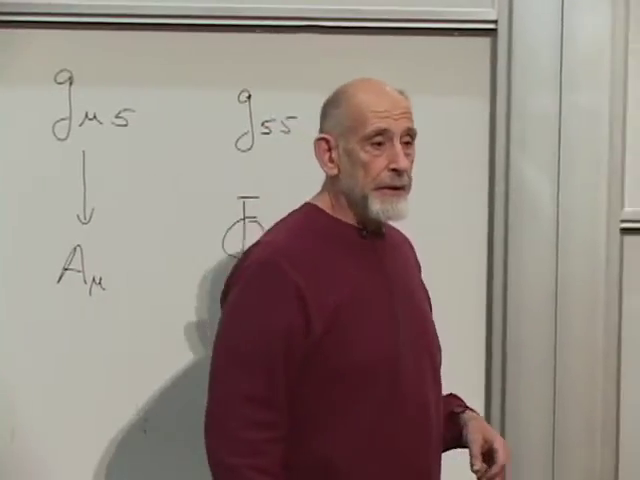
\includegraphics[width=0.72\textwidth]{lecture_10_figure_04.png}
  \caption{Le nombre quantique d’impulsion dans la direction compacte, tel qu’indiqué au tableau. Le cours représente schématiquement l’impulsion comme une intégrale de la vitesse dans cette direction.}
  \lectureframe{00:21:30}
  \label{fig:l10-compact-momentum-board}
\end{figure}

Une corde enroulée \(|w|\) fois a une longueur \(2\pi |w|R\). Avec une tension fondamentale de corde
\begin{equation}
  T_{\rm F}=\frac{1}{2\pi\alpha'},
\end{equation}
son énergie d’enroulement est
\begin{equation}
  E_{\rm wind}=T_{\rm F}(2\pi |w|R)
  =\frac{|w|R}{\alpha'}.
  \label{eq:l10-winding-energy}
\end{equation}
Dans les unités du cours, où \(\alpha'=1\), elle vaut simplement \(E_{\rm wind}=|w|R\).

Les deux tours de niveaux évoluent en sens opposés lorsque le rayon change. Pour \(R\gg
\sqrt{\alpha'}\), les niveaux d’impulsion sont rapprochés et ceux d’enroulement sont très espacés. Pour \(R\ll\sqrt{\alpha'}\), les niveaux d’impulsion sont très espacés et ceux d’enroulement sont rapprochés.

\begin{figure}[H]
  \centering
  \begin{minipage}[t]{0.48\textwidth}
    \centering
    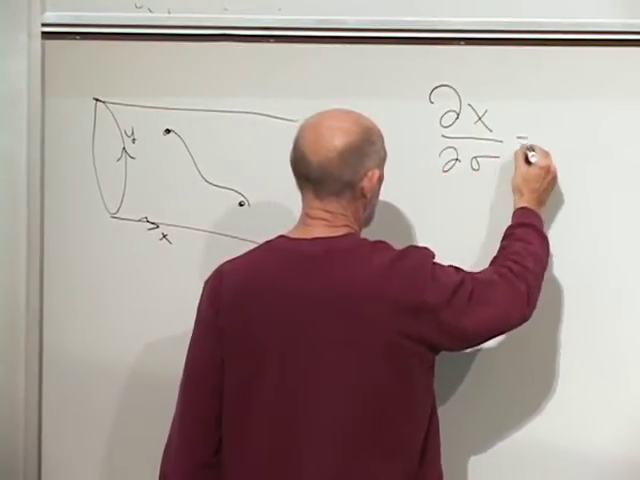
\includegraphics[width=\linewidth]{lecture_10_figure_05.png}
    \par\smallskip
    \textit{Grand rayon compact.}
  \end{minipage}\hfill
  \begin{minipage}[t]{0.48\textwidth}
    \centering
    \includegraphics[width=\linewidth]{lecture_10_figure_06.png}
    \par\smallskip
    \textit{Petit rayon compact.}
  \end{minipage}
  \caption{Les deux comparaisons spectrales présentées au tableau. Les tours clairsemés et denses échangent leurs rôles lorsque le rayon est inversé.}
  \lectureframe{00:25:30--00:26:00}
  \label{fig:l10-dual-spectra-board}
\end{figure}

Le schéma le plus simple est
\begin{figure}[H]
  \centering
  \begin{adjustbox}{max width=\linewidth}
  \begin{tikzpicture}[x=1cm,y=0.74cm,>=Latex]
    \node[font=\bfseries] at (-3.6,6.2) {$R\gg\sqrt{\alpha'}$};
    \draw[->] (-5.1,0) -- (-5.1,5.5) node[above] {$E$};
    \foreach \y in {0.4,1.0,1.6,2.2,2.8,3.4,4.0,4.6}
      \draw (-5.35,\y)--(-4.85,\y);
    \node[align=center] at (-4.25,5.15) {momentum\\dense};
    \draw[->] (-2.2,0) -- (-2.2,5.5) node[above] {$E$};
    \foreach \y in {0.4,2.4,4.4}
      \draw (-2.45,\y)--(-1.95,\y);
    \node[align=center] at (-1.35,5.15) {winding\\sparse};

    \node[font=\bfseries] at (3.6,6.2) {$R\ll\sqrt{\alpha'}$};
    \draw[->] (2.2,0) -- (2.2,5.5) node[above] {$E$};
    \foreach \y in {0.4,2.4,4.4}
      \draw (1.95,\y)--(2.45,\y);
    \node[align=center] at (3.05,5.15) {momentum\\sparse};
    \draw[->] (5.1,0) -- (5.1,5.5) node[above] {$E$};
    \foreach \y in {0.4,1.0,1.6,2.2,2.8,3.4,4.0,4.6}
      \draw (4.85,\y)--(5.35,\y);
    \node[align=center] at (5.95,5.15) {winding\\dense};
  \end{tikzpicture}
  \end{adjustbox}
  \caption{Reconstitution de l’argument fondé sur l’espacement des niveaux. Le spectre complet de la corde reste inchangé lorsque l’impulsion et l’enroulement sont échangés en même temps que \(R\leftrightarrow\alpha'/R\).}
  \label{fig:l10-dual-spectra-redraw}
\end{figure}

Supposons qu’on présente à un observateur l’un de ces spectres sans lui indiquer comment il a été obtenu. La tour de niveaux rapprochés correspond-elle à l’impulsion sur un grand cercle ou à l’enroulement sur un petit cercle ? Le spectre, à lui seul, ne permet pas de le dire. La théorie des cordes affirme plus fortement que les amplitudes de diffusion ne le permettent pas non plus. Les deux descriptions sont exactement équivalentes sous la transformation
\begin{equation}
  n\longleftrightarrow w,
  \qquad
  R\longleftrightarrow \widetilde R=\frac{\alpha'}{R}.
  \label{eq:l10-radius-duality}
\end{equation}
Le point fixe est
\begin{equation}
  R=\sqrt{\alpha'},
  \label{eq:l10-self-dual-radius}
\end{equation}soit \(R=1\) dans les unités du cours. À ce rayon, des états supplémentaires peuvent devenir sans masse et la symétrie de jauge est élargie.

\begin{classroomqa}
\audiencequestion{L’enroulement n’est-il qu’un artifice mathématique pour réécrire le spectre ? \lecturetimestamp{00:27:33}}
\lecturerresponse{Non. L’enroulement étiquette de véritables secteurs de l’espace de Hilbert de la corde fermée, et ces secteurs participent aux interactions. Le mot ``dualité'' signifie que les descriptions en termes d’impulsion et d’enroulement sont des coordonnées différentes d’une même physique, et non qu’un secteur n’est qu’un aide-mémoire facultatif pour l’autre.}
\end{classroomqa}

\begin{classroomqa}
\audiencequestion{Existe-t-il un rayon qui est envoyé sur lui-même ?
\lecturetimestamp{00:27:58}}
\lecturerresponse{Oui. La valeur auto-duale est
\(R=\sqrt{\alpha'}\), soit \(R=1\) dans les unités utilisées au tableau. Les deux tours se rejoignent en ce point, et le spectre présente une symétrie renforcée.}
\end{classroomqa}

\section{La forme de la dualité sur la feuille d’univers}

L’argument spectral est suggestif, mais la feuille d’univers rend l’échange plus précis. En jauge conforme, la quantité conjuguée à \(Y\) est proportionnelle à \(\partial_\tau Y\). L’impulsion compacte totale prend donc la forme
\begin{equation}
  P_Y=\frac{1}{2\pi\alpha'}
      \int_0^{2\pi}d\sigma\,\partial_\tau Y.
  \label{eq:l10-worldsheet-momentum}
\end{equation}
Le nombre d’enroulement vaut
\begin{equation}
  w=\frac{1}{2\pi R}
      \int_0^{2\pi}d\sigma\,\partial_\sigma Y
   =\frac{Y(2\pi)-Y(0)}{2\pi R}.
  \label{eq:l10-worldsheet-winding}
\end{equation}

\begin{classroomqa}
\audiencequestion{Pourquoi l’intégrale d’une dérivée ne s’annule-t-elle pas autour de la corde fermée ? \lecturetimestamp{00:32:33}}
\lecturerresponse{Parce que \(Y\) est une coordonnée périodique de l’espace cible, et non une fonction réelle univoque sur le cercle paramétré par \(\sigma\). Le point de la feuille d’univers \(\sigma=2\pi\) est identique à \(\sigma=0\), mais un relèvement de l’application d’immersion sur la droite de recouvrement varie de \(2\pi wR\). L’intégrale de \(\partial_\sigma Y\) mesure ce décalage.}
\end{classroomqa}

\begin{figure}[H]
  \centering
  \includegraphics[width=0.76\textwidth]{lecture_10_figure_07.png}
  \caption{Les intégrales de l’impulsion et de l’enroulement, une fois les deux lignes achevées au tableau. Les facteurs communs \(2\pi\) et \(\alpha'\) sont omis dans la normalisation du cours.}
  \lectureframe{00:33:25}
  \label{fig:l10-momentum-winding-integrals}
\end{figure}

Pour une corde enroulée une fois,
\begin{equation}
  Y(\tau,\sigma+2\pi)=Y(\tau,\sigma)+2\pi R.
\end{equation}
Pour un enroulement \(w\), le décalage du membre de droite vaut \(2\pi wR\). L’équation \eqref{eq:l10-worldsheet-winding} compte alors exactement l’enroulement. C’est la formulation précise de l’abréviation utilisée au tableau : \(w\sim R^{-1}\int
d\sigma\,\partial_\sigma Y\).

La formulation de la T-dualité sur la feuille d’univers est donc
\begin{equation}
  \partial_\tau Y\longleftrightarrow
  \partial_\sigma \widetilde Y,
  \qquad
  \partial_\sigma Y\longleftrightarrow
  \partial_\tau \widetilde Y,
  \label{eq:l10-derivative-duality}
\end{equation}
l’impulsion dans \(Y\) devenant l’enroulement dans la coordonnée duale \(\widetilde Y\), et réciproquement.

\begin{classroomqa}
\audiencequestion{Cela signifie-t-il que les coordonnées de la feuille d’univers \(\tau\) et \(\sigma\) sont elles-mêmes reliées ou échangées ?
\lecturetimestamp{00:34:39}}
\lecturerresponse{Non. La T-dualité associe des solutions et échange certaines dérivées de la coordonnée compacte de l’espace cible. Elle n’identifie pas la coordonnée temporelle de la feuille d’univers à sa coordonnée spatiale.}
\end{classroomqa}

\section{Pourquoi les états enroulés sont inévitables}

On peut se demander pourquoi une corde se trouverait dans un état enroulé alors qu’un état non enroulé est possible. Une corde ne choisit pas son état par préférence. L’énergie fournie lors d’une collision l’étire. Une corde suffisamment énergétique et fortement déformée peut se reconnecter en deux cordes d’enroulements opposés. Leur enroulement total reste nul, mais les deux cordes peuvent s’éloigner l’une de l’autre après la scission. L’une d’elles peut être envoyée très loin, laissant un observateur face à une corde enroulée apparemment isolée.

\begin{figure}[H]
  \centering
  \includegraphics[width=0.76\textwidth]{lecture_10_figure_08.png}
  \caption{Une configuration fortement étirée d’enroulement total nul, à partir de laquelle des cordes d’enroulements opposés peuvent s’éloigner après reconnexion.}
  \lectureframe{00:36:15}
  \label{fig:l10-winding-pair-production}
\end{figure}

Le seuil d’énergie est fixé par l’énergie d’enroulement. Sur un grand cercle, il faut une énergie de collision élevée pour étirer suffisamment la corde afin qu’elle fasse le tour de la direction compacte. Au-delà du seuil, cependant, la production de paires corde enroulée--anti-corde enroulée ne peut être interdite. L’analogie est celle de collisions de photons produisant une paire électron--positon. La charge électrique totale reste nulle, mais les particules chargées sont bien présentes et peuvent être séparées. La conservation de l’enroulement fonctionne de la même manière.

Cette analogie ne se limite pas aux mots. L’impulsion compacte et l’enroulement se comportent comme deux nombres quantiques de charge distincts. Dans la description réduite correspondante, les charges de même signe se repoussent et celles de signes opposés s’attirent. Il faut donc chercher les deux champs vectoriels qui transmettent ces forces.

\section{Charge d’impulsion issue de la gravitation en cinq dimensions}

Commençons par la gravitation en cinq dimensions. Les indices majuscules \(M,N\) parcourent les quatre directions ordinaires de l’espace-temps et la cinquième direction compacte. La métrique se décompose comme suit :
\begin{equation}
  G_{MN}\quad\longrightarrow\quad
  \bigl\{G_{\mu\nu},\,G_{\mu5},\,G_{55}\bigr\}.
  \label{eq:l10-metric-decomposition}
\end{equation}
La composante symétrique \(G_{5\mu}\) n’apporte aucune information nouvelle par rapport à \(G_{\mu5}\).

\begin{figure}[H]
  \centering
  \includegraphics[width=0.74\textwidth]{lecture_10_figure_09.png}
  \caption{Les groupes indépendants de composantes de la métrique en cinq dimensions : \(G_{\mu\nu}\), \(G_{\mu5}\) et \(G_{55}\).}
  \lectureframe{00:44:05}
  \label{fig:l10-metric-components}
\end{figure}

Du point de vue quadridimensionnel,
\begin{align}
  G_{\mu\nu} &\quad\hbox{is a spacetime metric},\\
  G_{\mu5} &\equiv A_\mu\quad\hbox{is a vector field},\\
  G_{55} &\equiv e^{2\varphi}\quad\hbox{is a scalar modulus}.
  \label{eq:l10-four-dimensional-fields}
\end{align}
Le scalaire \(\varphi\) mesure la taille de la direction compacte. Il peut varier de façon continue dans l’espace-temps ordinaire ; les ondes de \(\varphi\) sont donc des variations du rayon de la cinquième dimension.

\begin{figure}[H]
  \centering
  \includegraphics[width=0.74\textwidth]{lecture_10_figure_10.png}
  \caption{Au tableau, \(G_{\mu5}\) est identifié à un vecteur \(A_\mu\) et \(G_{55}\) à un scalaire \(\Phi\).}
  \lectureframe{00:47:40}
  \label{fig:l10-vector-and-radius-modulus}
\end{figure}

Une composante gravitationnelle mixte a pour source un flux d’impulsion mixte. En particulier, l’impulsion dans la cinquième direction source \(G_{\mu5}\). Un observateur quadridimensionnel interprète donc l’entier \(n\) comme une charge électrique couplée à \(A_\mu\). C’est le mécanisme de Kaluza--Klein : une quantité qui est une impulsion dans la géométrie de dimension supérieure devient une charge dans la théorie des champs de dimension inférieure.

\editorialnote{Dans le cours, le scalaire issu de \(G_{55}\) est appelé de façon approximative « ``dilaton'' ». Dans cette réduction, il s’agit précisément du module du rayon. Le dilaton de la corde en dix dimensions, qui détermine le couplage de la corde, est un champ distinct, même si des combinaisons scalaires de dimension inférieure peuvent se mélanger lors de changements de cadre et de dualité.}

\begin{classroomqa}
\audiencequestion{Le scalaire \(\varphi\) est-il proportionnel à l’entier d’impulsion \(n\) ? \lecturetimestamp{00:48:43}}
\lecturerresponse{Non. L’entier \(n\) étiquette un état quantifié et joue le rôle d’une charge. Le scalaire \(\varphi(x)\) est un champ continu qui détermine la taille locale de la compactification. Il peut varier d’un endroit à l’autre ; il n’est pas lui-même un entier.}
\end{classroomqa}

\section{Le second champ vectoriel et la charge d’enroulement}

L’enroulement se comporte lui aussi comme une charge, mais il ne peut pas se coupler de la même manière au même vecteur. Pour faire apparaître le second vecteur, revenons aux premières excitations de la corde fermée. Une corde fermée possède des modes oscillatoires gauches et droits. Les états physiques satisfont la condition d’appariement des niveaux : les niveaux totaux d’excitation gauche et droit doivent être égaux.

Dans la théorie bosonique, l’état non excité est le tachyon. Un oscillateur unique, gauche ou droit, ne satisferait pas l’appariement des niveaux. Le premier état sans masse autorisé contient donc un oscillateur de chaque type :
\begin{equation}
  \alpha_{-1}^{I}\widetilde\alpha_{-1}^{J}\ket{0;k}.
  \label{eq:l10-first-massless-state}
\end{equation}
Les indices \(I,J\) parcourent les directions spatiales transverses, y compris la direction compacte. Si l’un des indices correspond à une direction ordinaire et l’autre à \(5\), on obtient deux états d’oscillateur de type vectoriel :
\begin{equation}
  \alpha_{-1}^{\mu}\widetilde\alpha_{-1}^{5}\ket{0;k},
  \qquad
  \alpha_{-1}^{5}\widetilde\alpha_{-1}^{\mu}\ket{0;k}.
  \label{eq:l10-two-vector-states}
\end{equation}

\begin{figure}[H]
  \centering
  \includegraphics[width=0.76\textwidth]{lecture_10_figure_11.png}
  \caption{Les deux ordres d’oscillateurs gauche--droit qui deviennent des états vectoriels quadridimensionnels lorsqu’une polarisation pointe dans la direction compacte.}
  \lectureframe{00:58:20}
  \label{fig:l10-two-vector-states-board}
\end{figure}

Leurs combinaisons symétrique et antisymétrique appartiennent à des champs distincts de l’espace-temps :
\begin{align}
  \alpha_{-1}^{(\mu}\widetilde\alpha_{-1}^{5)}\ket{0;k}
    &\longleftrightarrow G_{\mu5},\\
  \alpha_{-1}^{[\mu}\widetilde\alpha_{-1}^{5]}\ket{0;k}
    &\longleftrightarrow B_{\mu5}.
  \label{eq:l10-g-and-b-vectors}
\end{align}
Le premier est le vecteur de Kaluza--Klein, dont la source est l’impulsion compacte. Le second provient du champ antisymétrique de Kalb--Ramond et a pour source l’enroulement de la corde. La théorie réduite contient donc deux champs analogues au photon, un pour chaque secteur de charge.

Si les deux indices de l’oscillateur pointent dans la direction compacte, l’état est un scalaire associé au module de compactification. S’ils pointent tous deux dans des directions transverses ordinaires, la partie symétrique sans trace est le graviton, la partie antisymétrique est \(B_{\mu\nu}\) et la trace contribue à un secteur scalaire.

\begin{classroomqa}
\audiencequestion{Lequel de ces états est le singulet et lequel est le triplet ? \lecturetimestamp{01:00:21}}
\lecturerresponse{Cette classification n’est pas pertinente ici. Les deux états mixtes se transforment comme des vecteurs quadridimensionnels. Leur somme et leur différence séparent la polarisation symétrique de la métrique de la polarisation antisymétrique du champ \(B\). L’état dont les deux indices sont compacts est, lui, un scalaire quadridimensionnel.}
\end{classroomqa}

Le dictionnaire complet établi avant la pause est le suivant :
\begin{equation}
  \boxed{
  \begin{gathered}
    n\leftrightarrow w,
    \qquad
    R\leftrightarrow\dfrac{\alpha'}{R},\\
    \partial_\tau Y\leftrightarrow\partial_\sigma\widetilde Y,
    \qquad
    G_{\mu5}\leftrightarrow B_{\mu5}.
  \end{gathered}}
  \label{eq:l10-complete-t-duality-map}
\end{equation}

\begin{figure}[H]
  \centering
  \includegraphics[width=0.72\textwidth]{lecture_10_figure_12.png}
  \caption{Récapitulatif au tableau de la transformation de T-dualité : l’impulsion et l’enroulement, le rayon et son inverse, les dérivées de la feuille d’univers et les deux champs vectoriels sont échangés. Le conférencier masque en partie la dernière ligne ; elle est donc donnée explicitement dans l’équation \eqref{eq:l10-complete-t-duality-map}.}
  \lectureframe{01:02:20}
  \label{fig:l10-t-duality-map-board}
\end{figure}

Cette construction ne doit pas être confondue avec l’affirmation que tous les champs énumérés ont déjà été identifiés dans le spectre observé des particules. À ce stade, il s’agit d’une conséquence mathématique de la théorie des cordes compactifiée. Il existe de nombreuses propositions pour relier de telles structures à la phénoménologie, mais ce n’est pas le problème traité dans ce cours.

\section{Les cordes ouvertes changent la question}

Après la pause, nous reprenons avec les cordes ouvertes. Une corde fermée peut avoir un enroulement stable, car elle n’a pas d’extrémité par laquelle celui-ci pourrait s’échapper. Une corde ouverte a des extrémités et ne possède donc pas d’enroulement analogue protégé topologiquement. Pourtant, la T-dualité est une symétrie exacte de la théorie. Que fait cette symétrie à une corde ouverte ?

Pour une extrémité libre de se déplacer, la variation de l’action de la corde donne une condition aux limites de Neumann. Dans la géométrie simple \((X,Y)\),
\begin{equation}
  \left.\partial_\sigma X\right|_{\partial\Sigma}=0,
  \qquad
  \left.\partial_\sigma Y\right|_{\partial\Sigma}=0.
  \label{eq:l10-neumann-boundary}
\end{equation}
L’interprétation mécanique est directe. Considérons la corde comme une chaîne composée d’éléments de masse de plus en plus petits. Une force tangentielle non nulle sur le dernier élément lui imprimerait une accélération qui diverge lorsque sa masse tend vers zéro. Une extrémité libre se déplace donc jusqu’à ce que la tension résultante à l’extrémité s’annule. On pourrait aussi maintenir l’extrémité fixe et fournir la force nécessaire, mais elle ne serait alors plus libre.

\begin{figure}[H]
  \centering
  \includegraphics[width=0.76\textwidth]{lecture_10_figure_13.png}
  \caption{La corde ouverte et ses conditions de Neumann aux extrémités, une fois complétées : \(\partial_\sigma X=\partial_\sigma Y=0\).}
  \lectureframe{01:09:20}
  \label{fig:l10-neumann-board}
\end{figure}

Effectuons maintenant la dualité uniquement sur la coordonnée compacte \(Y\). La coordonnée non compacte \(X\) reste inchangée. L’équation \eqref{eq:l10-derivative-duality} transforme la seconde condition de Neumann en
\begin{equation}
  \left.\partial_\tau\widetilde Y\right|_{\partial\Sigma}=0.
  \label{eq:l10-dirichlet-time-derivative}
\end{equation}
L’extrémité a donc une position indépendante du temps dans la direction compacte duale :
\begin{equation}
  \left.\widetilde Y\right|_{\partial\Sigma}=Y_0.
  \label{eq:l10-dirichlet-boundary}
\end{equation}
C’est une condition aux limites de Dirichlet.

\begin{figure}[H]
  \centering
  \includegraphics[width=0.76\textwidth]{lecture_10_figure_14.png}
  \medskip

  \begin{adjustbox}{max width=\linewidth}
  \begin{tikzpicture}[x=1cm,y=1cm,>=Latex]
    \node[align=center] at (-3.5,0.8)
      {Neumann\\\(\left.\partial_\sigma Y\right|_{\partial\Sigma}=0\)};
    \draw[->,thick] (-1.7,0.8) -- (1.3,0.8)
      node[midway,above] {$T_Y$};
    \node[align=center] at (3.4,0.8)
      {Dirichlet\\\(\left.\partial_\tau\widetilde Y\right|_{\partial\Sigma}=0\)};
    \node[align=center] at (3.4,-0.5)
      {\(\widetilde Y(\tau)=Y_0\) at each endpoint};
  \end{tikzpicture}
  \end{adjustbox}
  \caption{La condition complète imposée à l’extrémité duale, telle qu’écrite au tableau, et sa reconstruction logique. La T-dualité transforme la liberté de mouvement dans la direction compacte en une position fixe de l’extrémité dans la direction duale.}
  \lectureframe{01:12:35}
  \label{fig:l10-neumann-to-dirichlet}
\end{figure}

\begin{classroomqa}
\audiencequestion{Pourquoi la condition duale signifie-t-elle que l’extrémité est fixe ? \lecturetimestamp{01:12:39}}
\lecturerresponse{Parce que \(\partial_\tau\widetilde Y=0\) signifie que la vitesse dans la direction dualisée est nulle. Quelle que soit la position initiale de l’extrémité en \(\widetilde Y\), elle y reste. Ses coordonnées dans les directions parallèles non dualisées restent libres.}
\end{classroomqa}

\section{L’objet qui retient l’extrémité est une D-brane}

Si une extrémité est fixe, quelque chose doit pouvoir la maintenir en place. La T-dualité exacte exige donc un nouvel objet auquel les cordes ouvertes peuvent se terminer : une D-brane. La lettre \(D\) désigne Dirichlet, et non la dimension de l’objet. Dans l’anecdote historique racontée pendant le cours, ces objets auraient pu être nommés d’après Joseph Polchinski, dont l’analyse a rendu leur rôle dynamique indiscutable ; cependant, le terme déjà établi ``p-brane'' faisait de Dirichlet un nom naturel.

Une \(p\)-brane possède \(p\) dimensions spatiales. Une corde est une 1-brane, une membrane une 2-brane, et un objet étendu à trois dimensions une 3-brane. Une D\(p\)-brane est une \(p\)-brane sur laquelle les extrémités des cordes fondamentales satisfont des conditions de Dirichlet dans les directions transverses à la brane et des conditions de Neumann dans les directions qui lui sont tangentes.

Rien dans l’argument de dualité ne privilégie une valeur particulière de \(Y_0\) ; la D-brane ne peut donc pas être un élément rigide cloué en un point privilégié de l’univers. Elle doit pouvoir se déplacer. La relativité interdit aussi l’existence d’un corps étendu absolument rigide ; une D-brane peut donc fluctuer et se courber. La brane plane dessinée au tableau représente sa configuration d’équilibre, et non une restriction de sa dynamique.

\begin{classroomqa}
\audiencequestion{Les deux extrémités d’une corde ouverte doivent-elles avoir la même valeur fixe de la coordonnée duale ? \lecturetimestamp{01:14:55}}
\lecturerresponse{Pas en général. Les deux extrémités peuvent se trouver sur la même D-brane ; elles partagent alors la position transverse de celle-ci. Elles peuvent aussi se trouver sur deux D-branes différentes, situées à des positions transverses distinctes, auquel cas la corde s’étire entre elles. Une brane peut elle-même fluctuer et se courber ; le lieu des extrémités ne reste donc pas nécessairement un plan parfaitement plat.}
\end{classroomqa}

\section{Compter les dimensions d’une D-brane}

La théorie des supercordes en dix dimensions possède neuf dimensions spatiales. Supposons que la T-dualité impose une condition de Dirichlet dans une direction spatiale. L’extrémité reste libre dans les huit autres directions ; son lieu possible est donc une D8-brane de dimension huit. Chaque condition de Dirichlet indépendante supplémentaire supprime une direction de mouvement de l’extrémité. Si \(k\) coordonnées spatiales sont fixées, alors
\begin{equation}
  p=9-k.
  \label{eq:l10-dp-counting}
\end{equation}

La table illustre le même décompte en trois dimensions. Si l’on fixe la coordonnée verticale, le bout du doigt peut se déplacer sur une table bidimensionnelle. Si l’on fixe une deuxième coordonnée, il ne peut plus se déplacer que le long d’une ligne. Si l’on fixe les trois, il est confiné en un point.

\begin{figure}[H]
  \centering
  \begin{adjustbox}{max width=\linewidth}
  \begin{tikzpicture}[x=1.05cm,y=1cm,>=Latex]
    \draw[fill=blue!8] (-5.5,-0.7) -- (-2.5,-0.7) -- (-1.7,0.2)
      -- (-4.7,0.2) -- cycle;
    \node at (-3.6,-1.15) {one constraint: sheet};
    \draw[very thick,blue!60!black] (-0.9,-0.25) -- (1.3,-0.25);
    \node at (0.2,-1.15) {two constraints: line};
    \fill[blue!70!black] (4.1,-0.25) circle (0.09);
    \node at (4.1,-1.15) {three constraints: point};
    \draw[->] (-1.45,0.95) -- (-0.75,0.95);
    \draw[->] (2.25,0.95) -- (2.95,0.95);
    \node at (0.35,1.35) {each Dirichlet condition lowers \(p\) by one};
  \end{tikzpicture}
  \end{adjustbox}
  \caption{L’argument de décompte des dimensions illustré sur la table. Une D\(p\)-brane est le lieu où les extrémités restent libres de se déplacer.}
  \label{fig:l10-dp-counting-redraw}
\end{figure}

Des dualités répétées produisent des D8-, D7- et D6-branes, et ainsi de suite jusqu’à une D0-brane, ponctuelle dans l’espace. Si aucune direction spatiale n’est fixée, une D9-brane remplit les neuf dimensions spatiales et les cordes ouvertes ordinaires peuvent se déplacer partout. Le cours mentionne brièvement les D-branes D\((-1)\) : elles sont localisées dans l’espace-temps euclidien et se comportent comme des instantons plutôt que comme des particules ordinaires se propageant dans le temps.

\editorialnote{L’échelle des dimensions concerne les théories de type II considérées ensemble. Pour les D\(p\)-branes BPS stables, \(p\) est pair en type IIA et \(p\) impair en type IIB. La T-dualité le long d’un cercle modifie \(p\) d’une unité et échange simultanément les théories de type IIA et de type IIB.}

\begin{classroomqa}
\audiencequestion{Si seules six dimensions sont compactes, faut-il commencer le décompte en soustrayant de six plutôt que de neuf ? \lecturetimestamp{01:20:49}}
\lecturerresponse{La démonstration élémentaire applique la T-dualité aux directions compactes, mais le cercle dual devient arbitrairement grand lorsque le cercle initial devient arbitrairement petit. Dans cette limite, il est effectivement non compact. Les branes obtenues peuvent donc s’étendre dans des directions qui paraissent non compactes aux échelles accessibles, ou leur être transverses. La dimension \(p\) compte toutes les directions spatiales tangentes à la brane, et pas seulement les directions compactes utilisées dans une démonstration donnée.}
\end{classroomqa}

Une D0-brane est un nouveau type de particule. Une corde ouverte peut partir d’une D0-brane et se terminer sur une autre, revenir sur la même D0-brane ou s’étirer vers une brane très éloignée. Une corde allant littéralement jusqu’à l’infini spatial aurait une longueur et donc une énergie infinies ; dans la configuration physiquement utile, son autre extrémité se trouve sur un autre objet.

Le cas suivant, une D1-brane, a lui aussi la forme d’une corde, mais ce n’est pas la corde fondamentale par laquelle nous avons commencé. Elle peut se courber et se refermer sur elle-même, et des cordes fondamentales peuvent y prendre fin. Sa tension dépend du couplage des cordes d’une autre manière :
\begin{equation}
  T_{\rm D1}=\frac{1}{2\pi\alpha' g_s},
  \qquad
  T_{\rm F1}=\frac{1}{2\pi\alpha'}.
  \label{eq:l10-dstring-tension}
\end{equation}
À faible couplage \(g_s\ll1\), la corde D est beaucoup plus lourde que la corde fondamentale, ce qui explique qu’elle apparaisse d’abord comme un ancrage massif.

\begin{figure}[H]
  \centering
  \includegraphics[width=0.76\textwidth]{lecture_10_figure_15.png}
  \caption{La D1-brane du tableau : un objet unidimensionnel déformable, distinct des cordes fondamentales qui peuvent y prendre fin.}
  \lectureframe{01:24:20}
  \label{fig:l10-d1-brane}
\end{figure}

\begin{classroomqa}
\audiencequestion{La dualité T agit-elle sur les D-branes aussi bien que sur les cordes ? \lecturetimestamp{01:25:35}}
\lecturerresponse{Oui. Une dualité T parallèle à une D\(p\)-brane abaisse sa dimension à D\((p-1)\), tandis qu’une dualité T transverse à celle-ci l’élève à D\((p+1)\). Les branes font partie du dictionnaire de dualité ; elles ne sont pas des supports extérieurs que celle-ci laisserait inchangés.}
\end{classroomqa}

\begin{classroomqa}
\audiencequestion{Des directions tangentes à une brane peuvent-elles malgré tout être compactes ?
\lecturetimestamp{01:27:25}}
\lecturerresponse{Oui. ``Tangente'' et ``compacte'' répondent à des questions différentes. Une direction peut être parallèle à la brane tout en se refermant sur un cercle ; elle peut aussi être non compacte. Pour l’extrémité de la corde, ce qui importe, c’est que la condition aux limites dans cette direction soit de Neumann ou de Dirichlet.}
\end{classroomqa}

Une D2-brane est une membrane en forme de feuille. Une D3-brane a trois dimensions spatiales. Dans un espace-temps véritablement de dimension supérieure, une D3-brane est un sous-espace tridimensionnel et non la totalité de l’espace, même si les observateurs qui y sont confinés peuvent la percevoir comme l’ensemble de leur espace spatial.

\begin{figure}[H]
  \centering
  \includegraphics[width=0.76\textwidth]{lecture_10_figure_16.png}
  \caption{Une D2-brane représentée comme une feuille sur laquelle les extrémités des cordes peuvent se déplacer.}
  \lectureframe{01:27:55}
  \label{fig:l10-d2-brane}
\end{figure}

La dérivation présentée ici est volontairement schématique. À elle seule, elle ne prouve pas que la théorie des cordes décrit la nature. Au sein de la théorie des cordes, toutefois, les vérifications de cohérence sont nombreuses : les dualités, les calculs quantiques et les résultats mathématiques indiquent tous que les D-branes sont de véritables objets dynamiques.

\section{Les cordes ouvertes deviennent des champs sur une brane}

Considérons une D2-brane par ailleurs vide et plaçons-y de courtes cordes ouvertes. Chaque extrémité est confinée à la feuille, de sorte que toute excitation de basse énergie se déplace le long de celle-ci. Deux cordes orientées dont les extrémités adjacentes portent des flèches compatibles peuvent s’assembler. La corde ainsi formée peut ensuite se séparer de nouveau. Interprétés comme des trajectoires de particules, ces processus correspondent aux sommets des diagrammes de Feynman : deux particules entrent, une excitation intermédiaire se propage, puis deux particules ressortent.

\begin{figure}[H]
  \centering
  \includegraphics[width=0.76\textwidth]{lecture_10_figure_17.png}
  \caption{Des cordes ouvertes orientées sur une D2-brane s’assemblent lorsque leurs extrémités sont compatibles. À basse énergie, ce processus s’interprète comme une interaction de théorie des champs sur la brane.}
  \lectureframe{01:29:55}
  \label{fig:l10-open-strings-on-brane}
\end{figure}

À des énergies bien inférieures à l’échelle des cordes, la tour des modes vibrationnels internes n’est pas excitée. Il reste alors l’état sans masse de la corde ouverte, qui est un champ vectoriel sur le volume d’univers de la brane. Pour une seule brane, il s’agit d’un champ de jauge abélien \(U(1)\), l’analogue de l’électromagnétisme pour une brane. Le champ ne se propage pas dans tout le volume ambiant à dix dimensions ; ses quanta sont des cordes ouvertes dont les extrémités les maintiennent sur la brane.

\section{Un empilement de branes produit une couleur non abélienne}

Plaçons maintenant plusieurs branes parallèles à proximité les unes des autres. Pour trois branes, appelons-les Rouge, Vert et Bleu. Une corde orientée porte une paire ordonnée d’étiquettes à ses extrémités : elle peut aller de Rouge à Vert, de Vert à Bleu, de Rouge à Rouge, et ainsi de suite. Avec \(N\) branes, les états sans masse des cordes ouvertes peuvent être organisés en une matrice \(N\times N\)
\begin{equation}
  A_\mu{}^{i}{}_{j},
  \qquad i,j=1,\ldots,N.
  \label{eq:l10-chan-paton-matrix}
\end{equation}
Ce sont les étiquettes de Chan--Paton d’une théorie de jauge \(U(N)\).

\begin{figure}[H]
  \centering
  \includegraphics[width=0.76\textwidth]{lecture_10_figure_18.png}
  \medskip

  \begin{adjustbox}{max width=\linewidth}
  \begin{tikzpicture}[x=1cm,y=1cm,>=Latex]
    \draw[very thick,red!70!black] (-4.8,2.0)--(4.8,2.0);
    \draw[very thick,green!55!black] (-4.8,0.8)--(4.8,0.8);
    \draw[very thick,blue!70!black] (-4.8,-0.4)--(4.8,-0.4);
    \node[left] at (-4.8,2.0) {Red};
    \node[left] at (-4.8,0.8) {Green};
    \node[left] at (-4.8,-0.4) {Blue};
    \draw[->,thick] (-3.4,2.0) .. controls (-2.8,1.35) and (-2.3,1.15)
      .. (-1.7,0.8);
    \node at (-2.7,1.05) {$R\!G$};
    \draw[->,thick] (-0.6,0.8) .. controls (0.0,0.25) and (0.6,-0.05)
      .. (1.2,-0.4);
    \node at (0.1,0.0) {$G\!B$};
    \draw[->,thick] (2.1,2.0) .. controls (2.9,2.55) and (3.8,2.55)
      .. (4.3,2.0);
    \node at (3.2,2.65) {$R\!R$};
  \end{tikzpicture}
  \end{adjustbox}
  \caption{Trois branes parallèles au tableau et une reconstruction claire des étiquettes ordonnées des extrémités portées par les cordes qui les relient.}
  \lectureframe{01:33:15}
  \label{fig:l10-three-brane-stack}
\end{figure}

\begin{classroomqa}
\audiencequestion{Une corde peut-elle vraiment aller de la brane Rouge à la brane Verte sans être bloquée par les autres traits du dessin ? \lecturetimestamp{01:35:07}}
\lecturerresponse{Oui. Les branes sont plongées dans un espace de dimension supérieure. Le dessin sur un tableau à deux dimensions n’est qu’une projection ; une corde peut donc contourner un autre trait projeté en passant dans une direction transverse.}
\end{classroomqa}

\begin{classroomqa}
\audiencequestion{Une corde Rouge--Vert doit-elle s’assembler avec une corde Vert--Bleu pour devenir une corde Rouge--Bleu ? \lecturetimestamp{01:35:39}}
\lecturerresponse{C’est la règle fondamentale d’assemblage local. Des extrémités compatibles se rejoignent, et les deux segments forment une seule corde dont les extrémités libres conservent leurs étiquettes Rouge et Bleu. Les processus plus élaborés se construisent en répétant la même opération.}
\end{classroomqa}

La règle d’assemblage est la multiplication matricielle rendue géométrique. Une corde Rouge--Vert peut s’assembler avec une corde Vert--Bleu, car l’extrémité Verte de l’une est compatible avec l’extrémité Verte de l’autre. Le résultat est une corde Rouge--Bleu :
\begin{equation}
  (R,G)\circ(G,B)\longrightarrow(R,B).
  \label{eq:l10-color-composition}
\end{equation}
L’indice répété est raccordé et disparaît à l’intérieur. On retrouve cette même structure d’indices au sommet d’interaction de Yang--Mills.

\begin{figure}[H]
  \centering
  \includegraphics[width=0.76\textwidth]{lecture_10_figure_19.png}
  \caption{Assemblage de cordes ouvertes sur un empilement de branes. L’orientation des extrémités impose la même composition d’indices ordonnés que celle des champs de jauge non abéliens.}
  \lectureframe{01:36:30}
  \label{fig:l10-color-joining-board}
\end{figure}

Pour trois branes coïncidentes, le groupe de jauge complet des cordes ouvertes est \(U(3)\), avec neuf états vectoriels. Son algèbre se décompose ainsi :
\begin{equation}
  \mathfrak u(3)=\mathfrak{su}(3)\oplus\mathfrak u(1).
  \label{eq:l10-u3-decomposition}
\end{equation}
Les huit combinaisons sans trace ont la structure de couleur des gluons de la QCD, tandis que \(U(1)\), le centre de masse diagonal, est un champ abélien distinct.

\editorialnote{Le cours décrit l’une des neuf combinaisons de paires de couleurs comme pouvant se détacher et disparaître, ne laissant ainsi que huit gluons. La formulation précise pour les D-branes est qu’un empilement de trois branes coïncidentes donne \(U(3)\), et pas seulement \(SU(3)\). Pour obtenir l’octet de la QCD, il faut séparer, projeter ou découpler d’une autre manière le \(U(1)\) diagonal. L’image du cours illustre correctement les indices de couleur ordonnés, mais ne constitue pas une dérivation complète de la QCD.}

La matière de type quark porte un seul indice de couleur. Dans l’image des branes, elle est représentée par une corde dont une extrémité se trouve sur l’empilement de branes de couleur et l’autre sur une brane différente, éloignée. Par rapport à cet empilement, une seule extrémité porte une étiquette de couleur visible. L’inversion de l’orientation donne l’antiparticule. Une corde de type quark et une corde de type antiquark dont les extrémités sont compatibles peuvent s’assembler et quitter l’empilement de branes de couleur ; deux cordes de type quark ayant la même orientation ne peuvent pas s’annihiler de cette façon.

Les théories de basse énergie obtenues sont généralement des théories de Yang--Mills supersymétriques, avec de la matière supplémentaire déterminée par les branes et leurs intersections. Elles sont suffisamment proches de la QCD pour éclairer la dynamique non abélienne, mais elles ne sont pas automatiquement le Modèle standard. Avec une seule brane, la même construction se réduit à une théorie \(U(1)\) : les courtes cordes brane--brane sont analogues aux photons, tandis que les cordes orientées qui atteignent un second secteur jouent le rôle des charges électriques positives et négatives.

\section{Les cordes D prennent fin en monopoles magnétiques}

Il y a maintenant deux sortes d’objets de type corde dans cette histoire. La corde fondamentale, ou corde F, porte un flux électrique sur une D3-brane. La D1-brane, ou corde D, est beaucoup plus lourde à faible couplage. Une corde D peut elle aussi prendre fin sur une D3-brane. Son extrémité n’est pas chargée électriquement sous le champ de jauge du volume d’univers ; elle porte une charge magnétique. Pour les observateurs sur la D3-brane, cette extrémité est un monopole magnétique.

\begin{figure}[H]
  \centering
  \includegraphics[width=0.76\textwidth]{lecture_10_figure_20.png}
  \medskip

  \begin{adjustbox}{max width=\linewidth}
  \begin{tikzpicture}[x=1cm,y=1cm,>=Latex]
    \draw[fill=blue!7] (-3.8,-0.5)--(2.6,-0.5)--(3.6,0.35)--(-2.8,0.35)--cycle;
    \node at (2.25,-0.95) {D3-brane};
    \draw[very thick,red!70!black] (0.0,3.0)--(0.0,0.0);
    \fill[black] (0.0,0.0) circle (0.08);
    \node[right] at (0.15,2.1) {D-string};
    \foreach \a in {25,65,115,155} {
      \draw[->,blue!65!black] (0.0,0.0)--({1.25*cos(\a)},{0.65*sin(\a)});
    }
    \node[align=center] at (4.8,1.7) {magnetic flux\\on the D3 worldvolume};
    \draw[->] (3.7,1.35)--(1.05,0.45);
  \end{tikzpicture}
  \end{adjustbox}
  \caption{La construction du point d’extrémité au tableau et son interprétation précise. Une corde D qui prend fin sur une D3-brane apparaît comme un monopole magnétique pour la théorie de jauge du volume d’univers.}
  \lectureframe{01:41:30}
  \label{fig:l10-dstring-monopole}
\end{figure}

La hiérarchie des masses présente aussi la forme qualitative attendue. Puisque la tension de la corde D comporte un facteur \(1/g_s\), son extrémité est beaucoup plus lourde qu’une excitation électrique ordinaire à faible couplage. La relation électrique et magnétique entre les extrémités des cordes F et D fait partie de la structure plus vaste des dualités de la théorie des cordes de type IIB.

\begin{classroomqa}
\audiencequestion{L’extrémité de la corde D est-elle neutre ?
\lecturetimestamp{01:42:19}}
\lecturerresponse{Elle est neutre vis-à-vis de la charge électrique portée par une extrémité de corde fondamentale, mais elle n’est pas dépourvue de charge. Elle porte une charge magnétique et constitue donc un monopole dans la théorie de jauge de la D3-brane.}
\end{classroomqa}

\section{Ce que la construction affirme et ce qu’elle n’affirme pas}

Le chemin qui mène de la dualité T aux branes s’est construit au fil de plusieurs décennies, et non en un seul calcul. Une théorie d’abord proposée pour décrire les hadrons est devenue une théorie candidate de la gravité quantique. Ses dualités ont ensuite imposé la présence des D-branes dans le spectre, et les théories de jauge sont réapparues comme dynamique de basse énergie des cordes qui prennent fin sur ces branes. En ce sens, le sujet a bouclé la boucle.

Les D-branes et les constructions duales qui leur sont apparentées sont devenues de puissants outils pour étudier les théories de jauge supersymétriques, les systèmes fortement couplés et les liens entre gravité et théorie des champs. Elles ont également contribué à l’étude des fluides et des plasmas par l’intermédiaire de la dualité jauge/gravité. Ce succès ne revient pas à dériver directement le spectre observé des particules. Il reste à choisir la géométrie de compactification, la configuration des branes, la brisure de supersymétrie et de nombreux autres ingrédients.

\begin{classroomqa}
\audiencequestion{Qu’est-ce qui détermine la dimension compacte sur laquelle on effectue la dualité ?
\lecturetimestamp{01:44:59}}
\lecturerresponse{Mathématiquement, on peut effectuer la dualité sur toute direction compacte où la symétrie requise est présente, en choisissant la description la plus commode. Physiquement, les orientations des branes et les données de compactification réalisées dans un état donné sont déterminées par l’histoire et la dynamique de cet état.}
\end{classroomqa}

\begin{classroomqa}
\audiencequestion{Quelle brane intervient dans la construction du monopole ?
\lecturetimestamp{01:45:21}}
\lecturerresponse{L’espace dans lequel évolue la théorie de jauge est une D3-brane. La corde D s’étend dans une direction transverse et prend fin sur cette D3-brane ; son extrémité est le monopole observé dans les trois dimensions spatiales de la brane.}
\end{classroomqa}

\begin{classroomqa}
\audiencequestion{Les cordes D sont-elles elles aussi orientées ?
\lecturetimestamp{01:45:55}}
\lecturerresponse{Oui. Inverser l’orientation d’une corde D inverse la charge correspondante. Les deux orientations aux extrémités distinguent le monopole de l’antimonopole, tout comme l’orientation distingue les charges électriques aux extrémités des cordes fondamentales.}
\end{classroomqa}

\begin{classroomqa}
\audiencequestion{Cette représentation simple sur un tore peut-elle rendre compte de l’asymétrie gauche--droite de la physique chirale des particules ?
\lecturetimestamp{01:46:05}}
\lecturerresponse{Pas à elle seule. Un tore plat est trop symétrique. Les spectres chiraux exigent une structure supplémentaire, comme des intersections asymétriques de branes, des projections par orbifold ou une compactification sur des géométries de Calabi--Yau appropriées. La théorie des cordes dispose de mécanismes permettant d’obtenir la chiralité, mais ils dépassent le cadre de cette construction élémentaire fondée sur la dualité T.}
\end{classroomqa}

Nous avons suivi une même symétrie à travers quatre formes concrètes : un échange des spectres, un échange des dérivées sur la feuille d’univers, un échange des champs d’espace-temps et, enfin, un échange des conditions aux limites des extrémités. Cette dernière forme est décisive. Elle transforme une équivalence mathématique en découverte des D-branes, et la dynamique des cordes ouvertes en théorie de jauge sur leurs volumes d’univers. À ce stade, pour reprendre l’expression de Susskind, le cours a épuisé son temps, son énergie et sa quantité de mouvement.
